\documentclass[11pt]{article}

\usepackage[a4paper, margin=2.5cm]{geometry}
\usepackage[T1]{fontenc}
\usepackage[utf8]{inputenc}
\usepackage{lmodern}
\usepackage{microtype}
\usepackage{tikz}
\usetikzlibrary{shapes.geometric, arrows.meta, positioning, calc}
\usepackage{booktabs}
\usepackage{array}
\usepackage{enumitem}
\usepackage{titlesec}
\usepackage{graphicx}

% --- Simple, minimal styling (no colors) ---
\titleformat{\section}{\large\bfseries}{\thesection}{0.6em}{}
\titleformat{\subsection}{\normalsize\bfseries}{\thesubsection}{0.6em}{}
\setlength{\parindent}{0pt}
\setlength{\parskip}{0.5em}

\title{\textbf{Laporan Sistem WealthWise}\\[0.3em]
\large Software yang Digunakan, Arsitektur Sistem, Use Case, ERD, dan Flowchart}
\author{Tugas Besar -- Aplikasi Berbasis Platform}
\date{Juni 2026}

\begin{document}

% ===================== COVER =====================
\begin{titlepage}
\centering
\vspace*{2.5cm}

{\Large LAPORAN TUGAS BESAR}\\[0.2cm]
{\large Aplikasi Berbasis Platform -- Semester 6}\\[2.5cm]

{\Huge \textbf{WealthWise}}\\[0.4cm]
{\large Aplikasi Manajemen Keuangan Pribadi Berbasis AI}\\[2.5cm]

\begin{minipage}{0.8\textwidth}
\centering
Dokumen ini berisi:
\begin{itemize}[leftmargin=4cm]
\item Software / Teknologi yang Digunakan
\item Arsitektur Sistem
\item Use Case Diagram
\item Entity Relationship Diagram (ERD)
\item Flowchart Sistem
\end{itemize}
\end{minipage}

\vspace{3cm}

\textbf{Disusun oleh:}\\[0.4cm]
\begin{tabular}{ll}
Dhafin Ghiffary & 103012300348 \\
Fransiskus Harris Berliandu & 103012330401 \\
Alif Ihsan & 103012330079 \\
Mohammad Narendra Rasendriya Narayana & 103012300209 \\
Syauqi Nurfikri Rahman & 103012300299 \\
Yudha Setiawan Wicaksono & 103012300480 \\
\end{tabular}

\vfill
Juni 2026
\end{titlepage}

\tableofcontents
\newpage

% ===================== 1. SOFTWARE =====================
\section{Software yang Digunakan}

WealthWise dibangun dengan struktur \textit{monorepo} yang terdiri dari \textit{backend} (REST API) dan \textit{frontend} (Single Page Application), serta memanfaatkan layanan AI eksternal untuk fitur pintar. Berikut daftar perangkat lunak dan teknologi yang digunakan.

\subsection{Backend}
\begin{table}[h]
\centering
\begin{tabular}{@{}p{4cm}p{1.5cm}p{8cm}@{}}
\toprule
\textbf{Teknologi} & \textbf{Versi} & \textbf{Kegunaan} \\
\midrule
PHP & 8.2 & Bahasa pemrograman utama backend \\
Laravel & 12 & Framework untuk REST API \\
Laravel Sanctum & 4.0 & Autentikasi API berbasis token \\
SQLite / PostgreSQL & -- & Basis data \\
Guzzle HTTP & -- & Klien HTTP untuk komunikasi ke Groq API \\
\bottomrule
\end{tabular}
\end{table}

\subsection{Frontend}
\begin{table}[h]
\centering
\begin{tabular}{@{}p{4cm}p{1.5cm}p{8cm}@{}}
\toprule
\textbf{Teknologi} & \textbf{Versi} & \textbf{Kegunaan} \\
\midrule
React & 19 & Library untuk membangun antarmuka (UI) \\
Vite & 8 & Build tool dan dev server \\
Tailwind CSS & v4 & Styling berbasis utility class \\
React Router DOM & v7 & Routing pada sisi client \\
Recharts & 3.x & Visualisasi grafik dan statistik \\
Axios & -- & Klien HTTP untuk mengakses backend API \\
Lucide React & -- & Library ikon \\
\bottomrule
\end{tabular}
\end{table}

\subsection{Kecerdasan Buatan (AI)}
\begin{table}[h]
\centering
\begin{tabular}{@{}p{3cm}p{4.5cm}p{6cm}@{}}
\toprule
\textbf{Teknologi} & \textbf{Model} & \textbf{Kegunaan} \\
\midrule
Groq API & Llama 4 Scout 17B (Vision) & Receipt Scanner -- membaca struk belanja secara otomatis \\
Groq API & Llama 3.3-70B Versatile & Chatbot keuangan dan Daily Insight \\
\bottomrule
\end{tabular}
\end{table}

\subsection{DevOps dan Tools}
\begin{table}[h]
\centering
\begin{tabular}{@{}p{4cm}p{9.5cm}@{}}
\toprule
\textbf{Teknologi} & \textbf{Kegunaan} \\
\midrule
Docker + Apache & Containerization dan deployment \\
Composer & Manajemen dependency PHP \\
npm / Node.js & Manajemen dependency frontend \\
Laravel Pail & Log viewer real-time \\
concurrently & Menjalankan server, queue, dan Vite secara bersamaan \\
\bottomrule
\end{tabular}
\end{table}

\newpage
% ===================== 2. ARSITEKTUR SISTEM =====================
\section{Arsitektur Sistem}

WealthWise menggunakan arsitektur \textit{client-server} tiga lapis (3-tier):
\begin{enumerate}
\item \textbf{Frontend (Client Side)} -- Antarmuka pengguna tersedia dalam dua bentuk aplikasi: aplikasi mobile menggunakan \textbf{Flutter} dan aplikasi web menggunakan \textbf{React}. Keduanya berkomunikasi dengan backend melalui REST API dalam format JSON.
\item \textbf{Backend \& Logic} -- Backend \textbf{Laravel} menangani seluruh logika bisnis (controller dan service), validasi data, serta autentikasi menggunakan Laravel Sanctum (token-based).
\item \textbf{Data Store} -- Basis data \textbf{SQLite/PostgreSQL} menyimpan seluruh data pengguna, transaksi, kategori, target, dan notifikasi, diakses melalui Eloquent ORM.
\end{enumerate}

Selain ketiga lapisan di atas, backend juga terhubung ke \textbf{layanan AI eksternal (Groq API)} melalui HTTP request (Guzzle) untuk fitur \textit{receipt scanner}, \textit{chatbot}, dan \textit{daily insight}.

\begin{figure}[h]
\centering
\resizebox{\textwidth}{!}{%
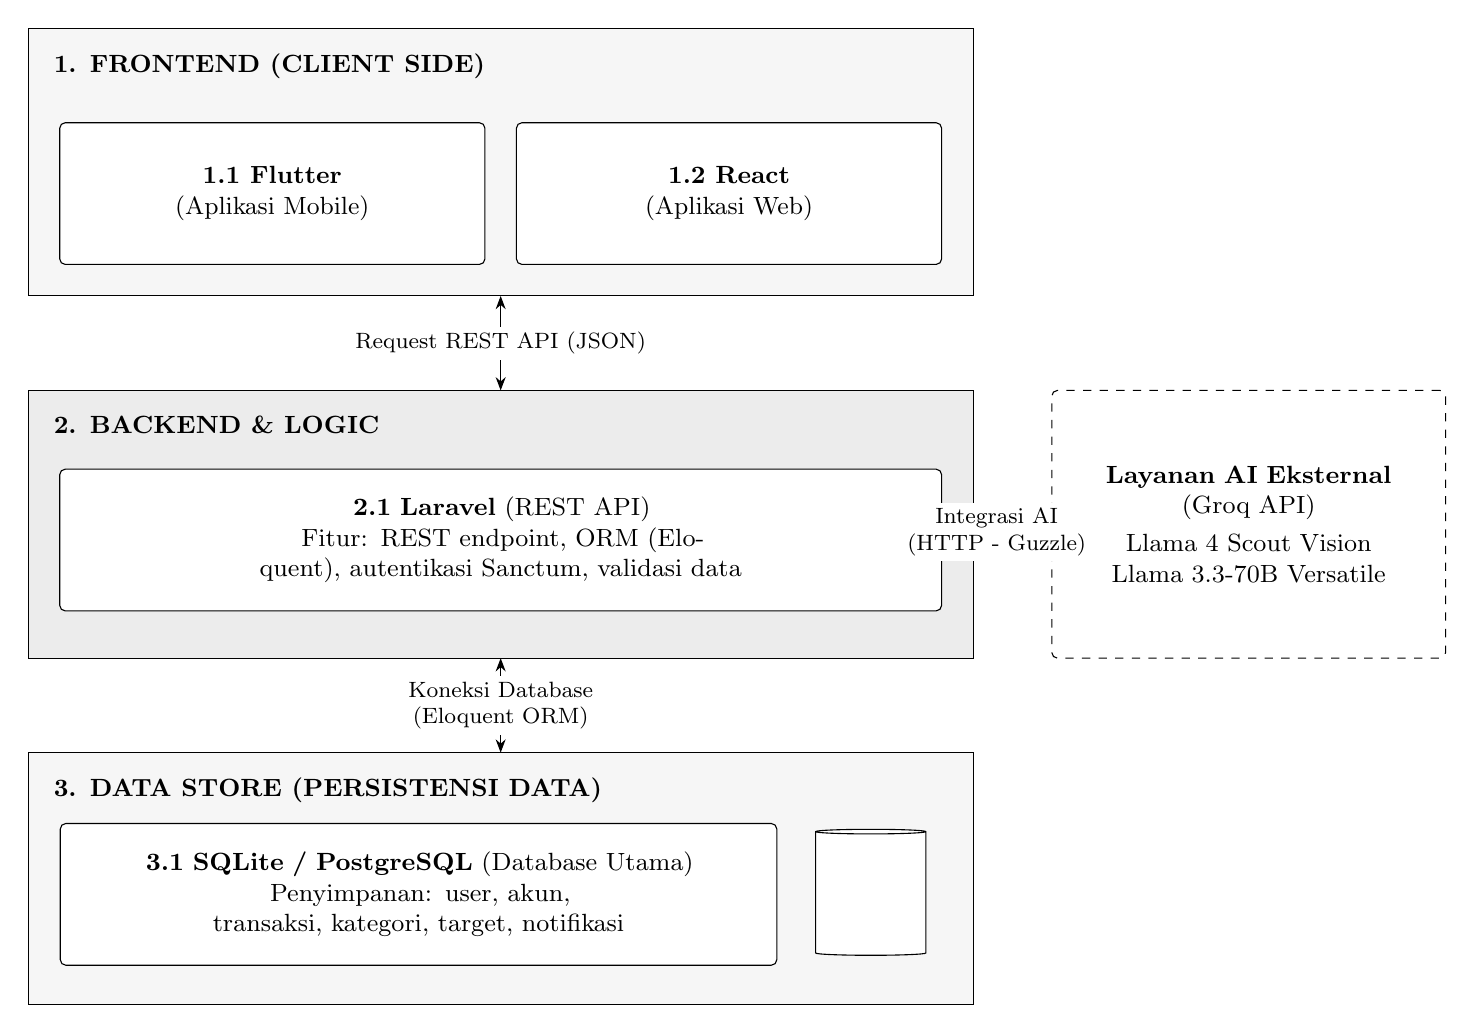
\begin{tikzpicture}[
  comp/.style={draw, rectangle, rounded corners=2pt, fill=white, align=center, font=\small},
  extbox/.style={draw, dashed, rectangle, rounded corners=2pt, fill=white, align=center, font=\small},
  lbl/.style={font=\footnotesize, align=center, fill=white, inner sep=2pt}
]

% ---- Layer 1: Frontend (Client Side) ----
\filldraw[fill=gray!7] (0,9.0) rectangle (12,12.4);
\node[anchor=north west, font=\small] at (0.2,12.2) {\textbf{1. FRONTEND (CLIENT SIDE)}};
\node[comp, minimum width=5.4cm, minimum height=1.8cm] (flutter) at (3.1,10.3) {\textbf{1.1 Flutter}\\ (Aplikasi Mobile)};
\node[comp, minimum width=5.4cm, minimum height=1.8cm] (react) at (8.9,10.3) {\textbf{1.2 React}\\ (Aplikasi Web)};

% ---- Layer 2: Backend & Logic ----
\filldraw[fill=gray!15] (0,4.4) rectangle (12,7.8);
\node[anchor=north west, font=\small] at (0.2,7.6) {\textbf{2. BACKEND \& LOGIC}};
\node[comp, minimum width=11.2cm, minimum height=1.8cm, text width=10.4cm] (laravel) at (6,5.9) {\textbf{2.1 Laravel} (REST API)\\ Fitur: REST endpoint, ORM (Eloquent), autentikasi Sanctum, validasi data};

% ---- Layer 3: Data Store ----
\filldraw[fill=gray!7] (0,0) rectangle (12,3.2);
\node[anchor=north west, font=\small] at (0.2,3.0) {\textbf{3. DATA STORE (PERSISTENSI DATA)}};
\node[comp, minimum width=9.1cm, minimum height=1.8cm, text width=8.4cm, anchor=west] (db) at (0.4,1.4) {\textbf{3.1 SQLite / PostgreSQL} (Database Utama)\\ Penyimpanan: user, akun, transaksi, kategori, target, notifikasi};
\node[cylinder, draw, shape border rotate=90, aspect=0.25, minimum width=1.4cm, minimum height=1.6cm, fill=white] (dbicon) at (10.7,1.4) {};

% ---- Layanan AI eksternal ----
\node[extbox, minimum width=5cm, minimum height=3.4cm, text width=4.4cm] (ai) at (15.5,6.1) {\textbf{Layanan AI Eksternal}\\ (Groq API)\\[0.3em] Llama 4 Scout Vision\\ Llama 3.3-70B Versatile};

% ---- Aliran data ----
\draw[{Stealth}-{Stealth}] (6,9.0) -- (6,7.8) node[lbl, midway] {Request REST API (JSON)};
\draw[{Stealth}-{Stealth}] (6,4.4) -- (6,3.2) node[lbl, midway] {Koneksi Database\\(Eloquent ORM)};
\draw[dashed, {Stealth}-{Stealth}] (laravel.east) -- (ai.west) node[lbl, midway] {Integrasi AI\\(HTTP - Guzzle)};

\end{tikzpicture}}
\caption{Arsitektur sistem WealthWise}
\end{figure}

\newpage
% ===================== 3. USE CASE =====================
\section{Use Case Diagram}

Aktor utama pada sistem WealthWise adalah \textbf{Pengguna}, yaitu pemilik akun yang telah login. Selain itu, terdapat aktor pendukung berupa \textbf{Layanan AI (Groq)} yang membantu beberapa proses tertentu.

\begin{figure}[h]
\centering
\resizebox{\textwidth}{!}{%
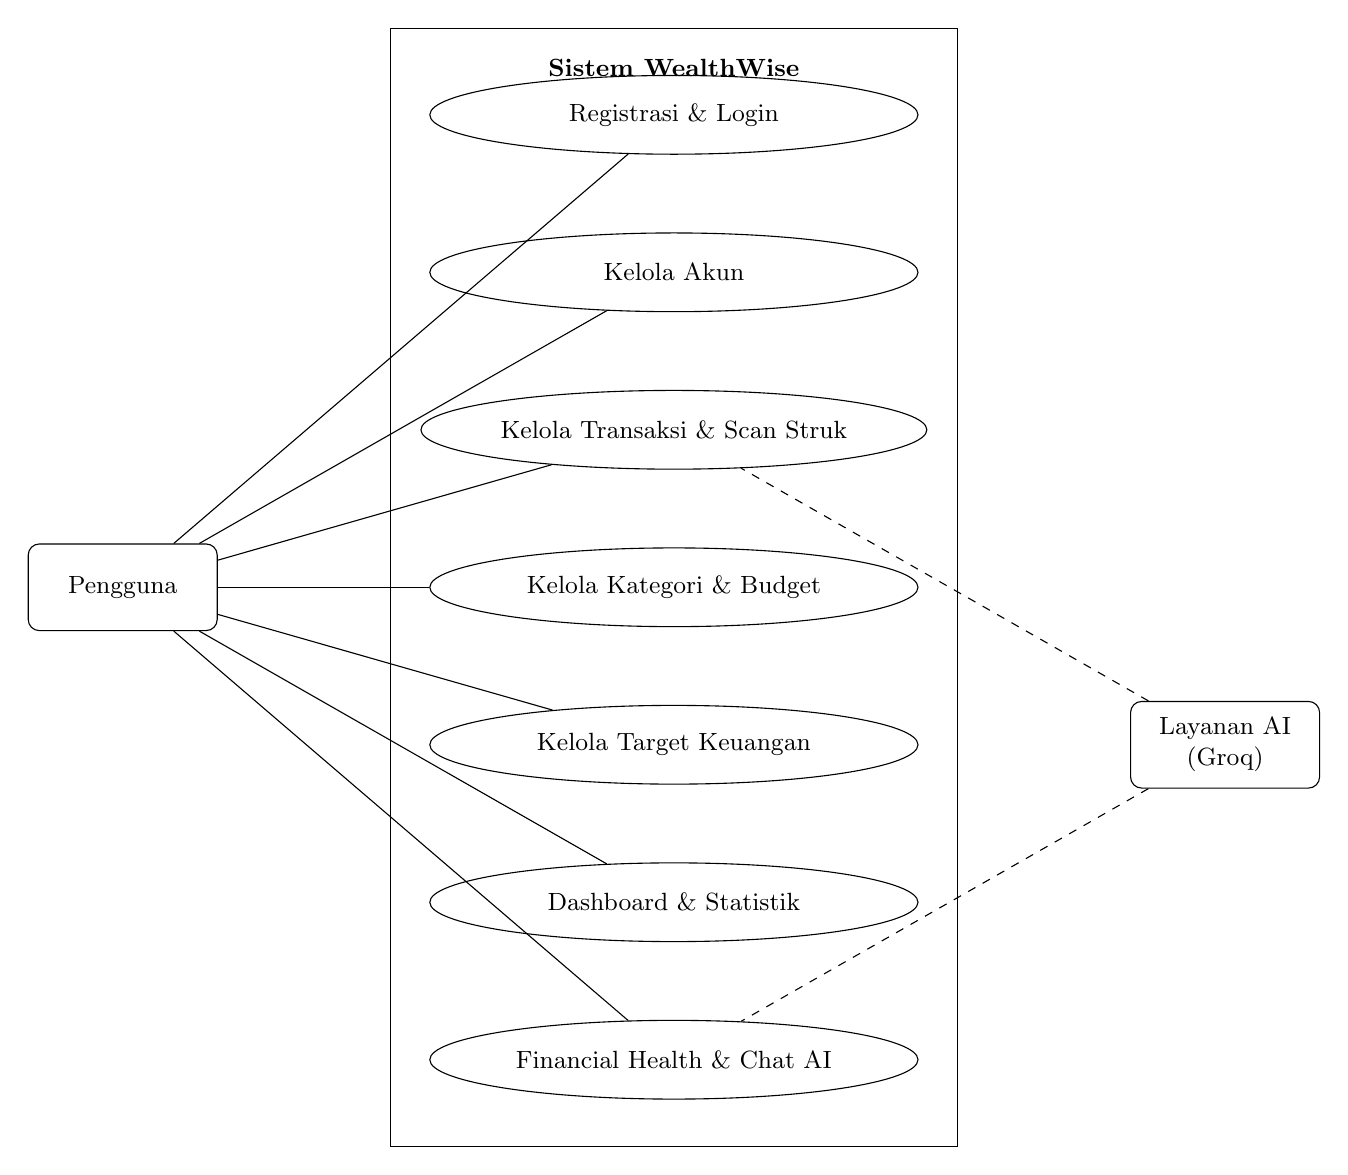
\begin{tikzpicture}[
  usecase/.style={draw, ellipse, minimum width=6.2cm, minimum height=1cm, align=center, font=\small, inner sep=2pt},
  actor/.style={draw, rectangle, rounded corners, minimum width=2.4cm, minimum height=1.1cm, align=center, font=\small}
]

% System boundary
\draw (3.4,13.1) rectangle (10.6,-1.1);
\node[font=\small] at (7,12.6) {\textbf{Sistem WealthWise}};

% Use cases (single column)
\node[usecase] (uc1) at (7,12) {Registrasi \& Login};
\node[usecase] (uc2) at (7,10) {Kelola Akun};
\node[usecase] (uc3) at (7,8)  {Kelola Transaksi \& Scan Struk};
\node[usecase] (uc4) at (7,6)  {Kelola Kategori \& Budget};
\node[usecase] (uc5) at (7,4)  {Kelola Target Keuangan};
\node[usecase] (uc6) at (7,2)  {Dashboard \& Statistik};
\node[usecase] (uc7) at (7,0)  {Financial Health \& Chat AI};

% Actors
\node[actor] (userActor) at (0,6) {Pengguna};
\node[actor] (aiActor) at (14,4) {Layanan AI\\(Groq)};

% Connections from user actor to all use cases
\foreach \i in {1,...,7} {
  \draw (userActor) -- (uc\i);
}

% AI actor connections (dashed) -- fitur yang melibatkan AI
\draw[dashed] (aiActor) -- (uc3);
\draw[dashed] (aiActor) -- (uc7);

\end{tikzpicture}}
\caption{Use case diagram WealthWise}
\end{figure}

\newpage
\subsection{Deskripsi Use Case}
\begin{table}[h]
\centering
\begin{tabular}{@{}p{4.5cm}p{9cm}@{}}
\toprule
\textbf{Use Case} & \textbf{Deskripsi} \\
\midrule
Registrasi \& Login & Pengguna mendaftar, login, dan memverifikasi email menggunakan kode 6 digit. Autentikasi berbasis token (Sanctum). \\
Kelola Akun & Menambah, melihat, mengubah, dan menghapus akun (Bank, E-Wallet, Tunai, dll.) beserta saldonya. \\
Kelola Transaksi \& Scan Struk & Mencatat pemasukan, pengeluaran, dan transfer antar akun. Mendukung scan struk belanja otomatis menggunakan AI (OCR). \\
Kelola Kategori \& Budget & Membuat kategori transaksi kustom dan menetapkan batas budget per periode (mingguan/bulanan/tahunan). \\
Kelola Target Keuangan & Membuat target tabungan (Smart Planning) dengan rencana pengisian harian/mingguan/bulanan dan memantau progresnya. \\
Dashboard \& Statistik & Menampilkan ringkasan saldo, grafik pemasukan/pengeluaran, dan transaksi terbaru. \\
Financial Health \& Chat AI & Menampilkan skor kesehatan keuangan, insight harian, dan chatbot yang menjawab berdasarkan data finansial pengguna. \\
\bottomrule
\end{tabular}
\end{table}

\newpage
% ===================== 4. ERD =====================
\section{Entity Relationship Diagram (ERD)}

Struktur basis data WealthWise terdiri dari tabel \texttt{users} sebagai entitas utama yang terhubung dengan entitas \texttt{accounts}, \texttt{categories}, \texttt{transactions}, \texttt{financial\_goals}, \texttt{insights}, dan \texttt{notifications}. Tabel \texttt{transactions} merupakan entitas penghubung yang mencatat aliran dana antar akun dan kategori.

\begin{figure}[h]
\centering
\resizebox{\textwidth}{!}{%
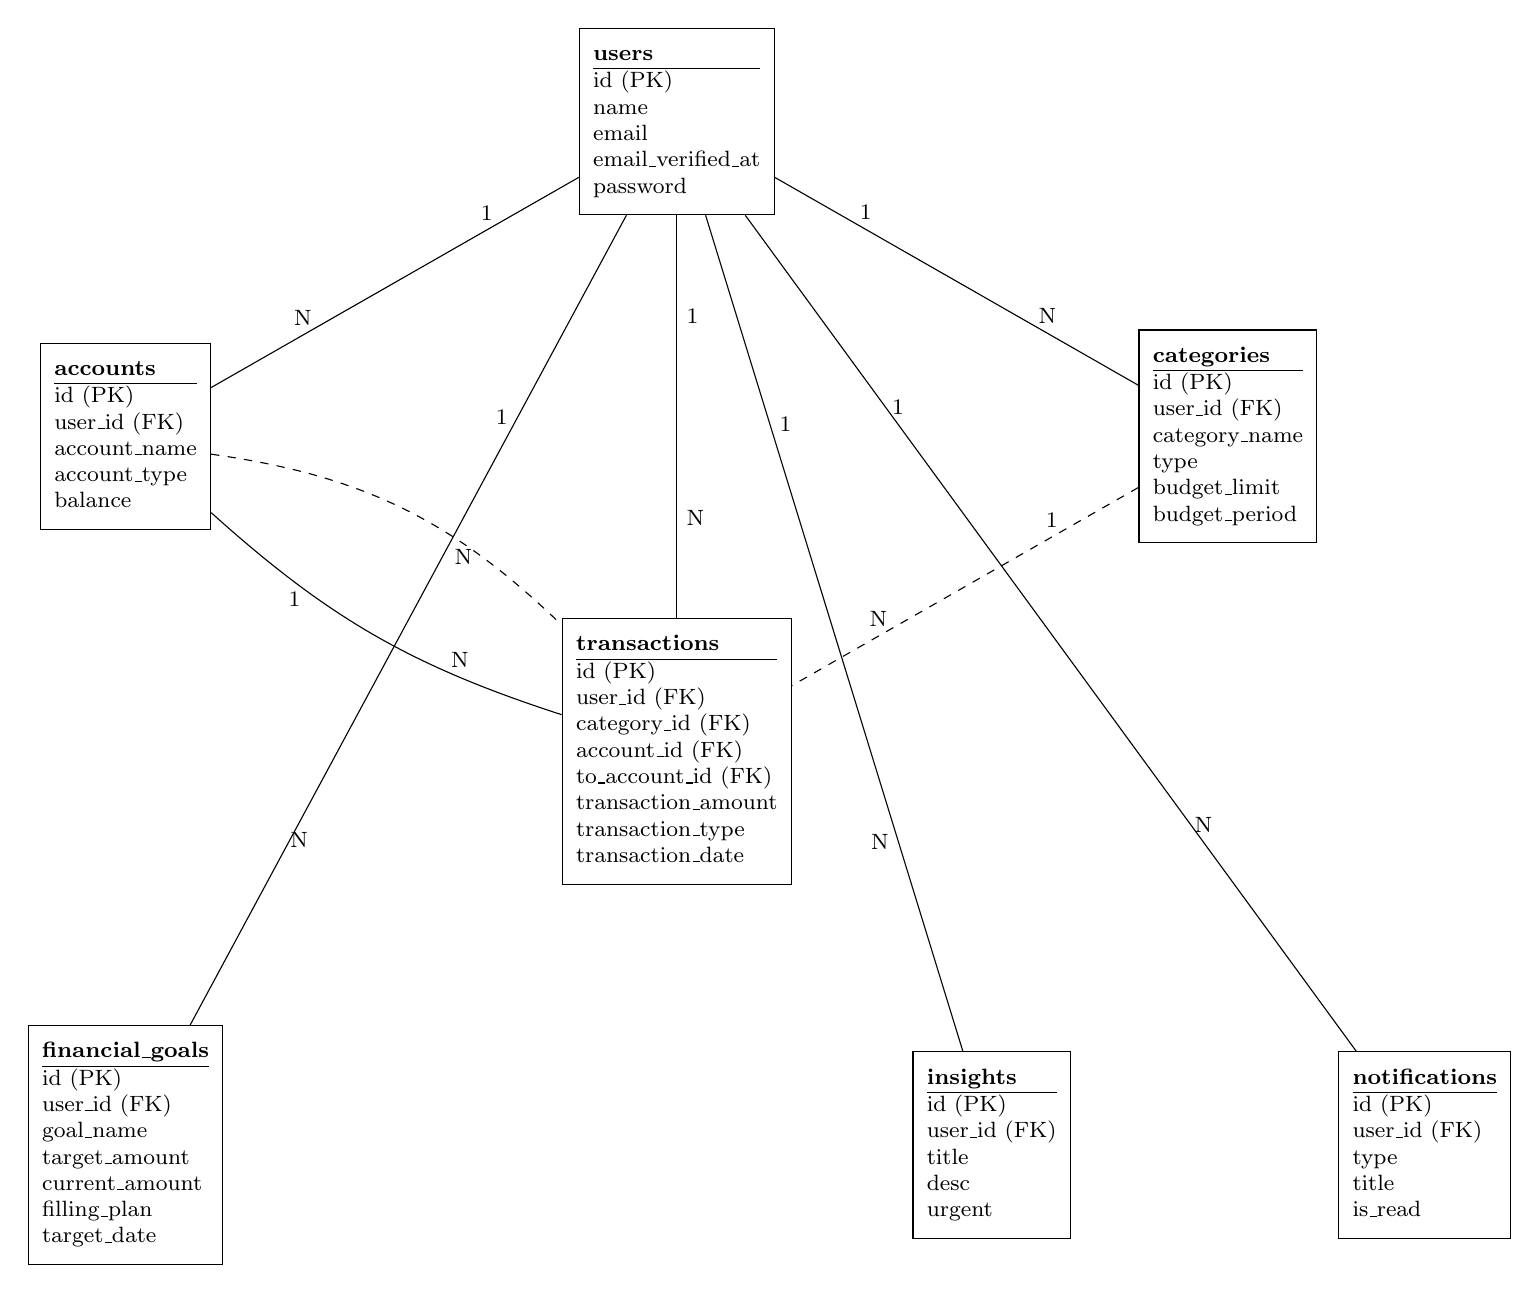
\begin{tikzpicture}[
  entity/.style={draw, align=left, font=\footnotesize, inner sep=5pt},
  rel/.style={font=\footnotesize}
]

\node[entity] (users) at (8,15) {%
\begin{tabular}{@{}l@{}}
\textbf{users}\\\hline
id (PK)\\
name\\
email\\
email\_verified\_at\\
password
\end{tabular}};

\node[entity] (accounts) at (1,11) {%
\begin{tabular}{@{}l@{}}
\textbf{accounts}\\\hline
id (PK)\\
user\_id (FK)\\
account\_name\\
account\_type\\
balance
\end{tabular}};

\node[entity] (categories) at (15,11) {%
\begin{tabular}{@{}l@{}}
\textbf{categories}\\\hline
id (PK)\\
user\_id (FK)\\
category\_name\\
type\\
budget\_limit\\
budget\_period
\end{tabular}};

\node[entity] (transactions) at (8,7) {%
\begin{tabular}{@{}l@{}}
\textbf{transactions}\\\hline
id (PK)\\
user\_id (FK)\\
category\_id (FK)\\
account\_id (FK)\\
to\_account\_id (FK)\\
transaction\_amount\\
transaction\_type\\
transaction\_date
\end{tabular}};

\node[entity] (goals) at (1,2) {%
\begin{tabular}{@{}l@{}}
\textbf{financial\_goals}\\\hline
id (PK)\\
user\_id (FK)\\
goal\_name\\
target\_amount\\
current\_amount\\
filling\_plan\\
target\_date
\end{tabular}};

\node[entity] (insights) at (12,2) {%
\begin{tabular}{@{}l@{}}
\textbf{insights}\\\hline
id (PK)\\
user\_id (FK)\\
title\\
desc\\
urgent
\end{tabular}};

\node[entity] (notifications) at (17.5,2) {%
\begin{tabular}{@{}l@{}}
\textbf{notifications}\\\hline
id (PK)\\
user\_id (FK)\\
type\\
title\\
is\_read
\end{tabular}};

% Relasi dari users (1) ke entitas anak (N)
\draw (users) -- (accounts) node[rel, near start, above]{1} node[rel, near end, above]{N};
\draw (users) -- (categories) node[rel, near start, above]{1} node[rel, near end, above]{N};
\draw (users) -- (transactions) node[rel, near start, right]{1} node[rel, near end, right]{N};
\draw (users) -- (goals) node[rel, near start, left]{1} node[rel, near end, below]{N};
\draw (users) -- (insights) node[rel, near start, right]{1} node[rel, near end, left]{N};
\draw (users) -- (notifications) node[rel, near start, above]{1} node[rel, near end, above]{N};

% Relasi accounts -- transactions (akun sumber dan akun tujuan)
\draw (accounts) to[bend right=12] node[rel, near end, above]{N} node[rel, near start, below]{1} (transactions);

\draw[dashed] (accounts) to[bend left=18] node[rel, near end, left]{N} (transactions);

% Relasi categories -- transactions
\draw[dashed] (categories) -- (transactions) node[rel, near start, above]{1} node[rel, near end, above]{N};

\end{tikzpicture}}
\caption{Entity Relationship Diagram (ERD) WealthWise}
\end{figure}

\subsection{Keterangan Relasi}
\begin{itemize}
\item Satu \texttt{user} dapat memiliki banyak \texttt{accounts}, \texttt{categories}, \texttt{transactions}, \texttt{financial\_goals}, \texttt{insights}, dan \texttt{notifications} (relasi 1:N).
\item Satu \texttt{transaction} merujuk ke satu \texttt{account} sebagai akun sumber (\texttt{account\_id}), dan secara opsional ke satu \texttt{account} lain sebagai akun tujuan (\texttt{to\_account\_id}) untuk transaksi bertipe \texttt{TRANSFER}.
\item Satu \texttt{category} dapat memiliki banyak \texttt{transactions} (\texttt{category\_id} bersifat opsional / nullable).
\end{itemize}

\newpage
% ===================== 5. FLOWCHART =====================
\section{Flowchart Sistem}

Flowchart berikut menggambarkan alur penggunaan aplikasi WealthWise secara umum, mulai dari membuka aplikasi, autentikasi, hingga penggunaan fitur-fitur utama secara berulang sampai pengguna logout.

\begin{figure}[h]
\centering
\resizebox{!}{0.85\textheight}{%
\begin{tikzpicture}[
  startend/.style={draw, ellipse, minimum width=2.6cm, minimum height=1cm, align=center, font=\small},
  proc/.style={draw, rectangle, minimum width=4.6cm, minimum height=1cm, align=center, font=\small},
  dec/.style={draw, diamond, aspect=3, minimum width=4.4cm, minimum height=1.2cm, align=center, font=\small, inner sep=2pt},
  lbl/.style={font=\footnotesize}
]

\node[startend] (mulai) at (0,18) {Mulai};
\node[proc] (akses) at (0,16.5) {Buka Aplikasi WealthWise};
\node[dec] (cekAkun) at (0,14.5) {Sudah punya\\akun?};
\node[proc] (registrasi) at (-6.6,14.5) {Registrasi \& Verifikasi Email (kode 6 digit)};
\node[proc] (login) at (0,12) {Login};
\node[dec] (cekLogin) at (0,10) {Login\\berhasil?};
\node[proc] (dashboard) at (0,8) {Tampil Dashboard Utama};
\node[proc] (pilihMenu) at (0,6.3) {Pilih Menu Fitur};
\node[proc] (proses) at (0,4.3) {Sistem Memproses \& Menampilkan Hasil};
\node[dec] (cekLanjut) at (0,2.3) {Lanjut\\pakai\\aplikasi?};
\node[proc] (logout) at (0,0) {Logout};
\node[startend] (selesai) at (0,-1.5) {Selesai};

% Arrows - main flow
\draw[-{Stealth}] (mulai) -- (akses);
\draw[-{Stealth}] (akses) -- (cekAkun);
\draw[-{Stealth}] (cekAkun) -- node[lbl, right]{Ya} (login);
\draw[-{Stealth}] (login) -- (cekLogin);
\draw[-{Stealth}] (cekLogin) -- node[lbl, right]{Ya} (dashboard);
\draw[-{Stealth}] (dashboard) -- (pilihMenu);
\draw[-{Stealth}] (pilihMenu) -- (proses);
\draw[-{Stealth}] (proses) -- (cekLanjut);
\draw[-{Stealth}] (cekLanjut) -- node[lbl, right]{Tidak} (logout);
\draw[-{Stealth}] (logout) -- (selesai);

% Registrasi branch (Tidak)
\draw[-{Stealth}] (cekAkun) -- node[lbl, above]{Tidak} (registrasi);
\draw[-{Stealth}] (registrasi) |- (login.west);

% Login gagal -> kembali ke Login
\draw[-{Stealth}] (cekLogin.east) -- ++(2.4,0) |- node[lbl, pos=0.27, right]{Tidak} (login.east);

% Lanjut pakai aplikasi -> kembali ke Pilih Menu
\draw[-{Stealth}] (cekLanjut.west) -- ++(-2.6,0) |- node[lbl, pos=0.27, above]{Ya} (pilihMenu.west);

\end{tikzpicture}}
\caption{Flowchart alur penggunaan aplikasi WealthWise}
\end{figure}

\textit{Pilih Menu Fitur} pada flowchart di atas mewakili menu-menu utama aplikasi, yaitu: Kelola Akun, Kelola Transaksi (termasuk Scan Struk AI), Kelola Kategori \& Budget, Kelola Target Keuangan, Statistik, dan Financial Health.

\end{document}
